\documentclass[12pt]{article}
\usepackage{multicol}
\usepackage{apacite}
\usepackage{graphicx}
\usepackage{setspace}
\usepackage{amsmath}
\usepackage{mathtools}
\usepackage{fixltx2e}
\DeclareGraphicsExtensions{.pdf,.svg,.png,.jpg}

% title page
\begin{document}
\title{Visualizing and Refining Connectivity Map Query Results}
\maketitle
\begin{titlepage}
\begin{center}
Proposal for a\\
Thesis in the Field of\\
Biotechnology\\[\baselineskip]
In Partial Fulfillment of the Requirements\\
for a Master of Liberal Arts Degree\\[\baselineskip]
Harvard University\\
Extension School\\[\baselineskip]
Theodore Natoli\\
51 Lewis Avenue, Apartment 3\\
Arlington, MA 02472\\
857-498-1946\\
\texttt{tnatoli@fas.harvard.edu}\\[\baselineskip]
Proposed Start Date: \today\\
Anticipated Date of Graduation: \today\\
Thesis Director: Aravind Subramanian
\end{center}
\end{titlepage}
% end of title stuff

\begin{abstract}
The Connectivity Map (CMap) is a database of gene expression signatures obtained from experiments in which cultured human cells are treated with pharmacologic and genomic perturbagens. A typical use case of this database is for a researcher to query with a signature of a cell state of interest and use the matching perturbagens to develop a functional hypothesis for follow-up. Current pattern matching algorithms that perform CMap queries suffer from a universal weakness -- the enormous size and richness of signatures in CMap means that a query typically generates hundreds of strong connections. These connections are hard to distinguish, thereby making prioritization difficult. I hypothesize that one mode of prioritization is to highlight query results that are highly interconnected amongst themselves over singletons. The goal of this work is to provide a web-based tool for implementing an interconnectivity-based method of query result refinement and for visualizing CMap query results in a graph layout.
\end{abstract}

% begin double spacing
\doublespacing

\section{The Research Problem}

The CMap database is a compendium of gene expression signatures resulting from the treatment of cultured human cells with small molecule compounds (CP), short hairpin RNAs (shRNA), or over-expression constructs (OE). The utility of the CMap database is that of a gene expression search engine. Users are able to pose questions about relationships between cellular states and formulate hypotheses based on similarities or differences in the states' gene expression signatures.

Hypotheses are generated by posing search queries into the database and examining the query results. A CMap query is a focused question in which a user inputs a gene expression signature, called the query, and computes the similarity, or connectivity, between his/her query and other signatures in the database. Positive connectivity indicates that two signatures' expression changes are similar and vice versa. Researchers can use CMap to find connections between signatures within or external to the database. Hypotheses may be in the form of ``the shRNA knockdown of gene X connects to shRNA knockdown signatures of pathway Y members, so X is probably a member of Y.'' Or perhaps ``the signature of compound Z connects to the knockdown signature of gene X, so perhaps X is the target of Z''.

Lamb et al demonstrated a more directly therapeutically relevant use of the original incarnation of CMap when they discovered that the signature of sirolimus connected strongly to a signature of dexamethasone sensitivity. Dexamethasone is a treatment for acute lymphoblastic leukemia (ALL), but many patients eventually become resistant \cite{tissing_molecular_2003}. The CMap connection between sirolimus and dexamathasone sensitivity suggested that sirolimus might be effective in reversing resistance in ALL patients who had become resistant to dexamethasone. A follow-up experiment confirmed that sirolimus conferred dexamathasone sensitivity to CEM-c1 cells, a previously dexamethasone-resistant cell line \cite{lamb_connectivity_2006}. 

The CMap database contains over 400,000 signatures spanning over 70 cell types. Because of the large size of the CMap database, interpreting and prioritizing query results has become a difficult task. For example, accepting only the top one percent of connections yields nearly 4,000 signatures. Follow-up on such a large number of primary hits is nearly impossible in most cases. I propose that within a set of initial query results, there will frequently exist a set or sets of signatures that are more tightly interconnected with themselves than with other signatures. These interconnected sets are more likely to be indicative of robust biological signal and should therefore be prioritized over other singleton connections. The goal of this work is to build a web-based tool to implement an algorithm to identify subsets of high interconnectivity with lists of initial query results and to visualize the relationships between these subsets in a graph layout. I propose that this tool will be useful in refining initial CMap query results into smaller, more actionable lists of connections that can be further investigated in secondary assays.

% key terms
\section{Key Terms}
\begin{enumerate}
\item gene expression profiling:
\item gene set enrichment analysis (GSEA):
\item Kolmogorov-Smirnov (KS) statistic:
\item graphical model:
\item CMap connection: 
\end{enumerate}

% background
\section{Background}
\subsection{Gene Expression Profiling}

Gene expression profiling is the simultaneous measure of the RNA transcript levels of many genes within a cell or group of cells. These measurements can help to provide insight into the cellular state or states of the cells in question. For example, if many cell-cycle genes are observed to be active, it could suggest that the cells are actively dividing. Conversely, if many apoptotic genes are active, the cells might be dying. Frequently, the goal of gene expression profiling is to identify genes that are differentially regulated between one or more sets of conditions. For example, one might measure expression in cells that have and have not been treated with a drug of interest, and then compare the resulting expression profiles to identify genes that are substantially up- or down-regulated in the treated cells relative to the untreated. Current technology, such as the microarray, allow for many such gene expression experiments to be run in parallel, enabling the comparative analysis of hundreds or thousands of expression profiles corresponding to an equal number of experimental conditions. Similarly, expression profiling can be used to identify genes differentially regulated between disease and normal states. van't Veer et al used gene expression profiling to identify a set of genes, that were predictive of breast cancer metastasis \cite{van_t_veer_gene_2002}. Because of its ability to identify such signatures, gene expression profiling is a powerful and often-used tool in contemporary biology.

\subsection{Gene Set Enrichment Analysis (GSEA)}

Gene Set Enrichment Analysis (GSEA) is an analytical approach designed to extract biological insight from gene expression data \cite{subramanian_gene_2005}. It leverages  groups of genes, called gene sets, that share some biological commonality (i.e. members of a cellular signaling pathway) and computes their enrichment, or trend towards the top or bottom, of a ranked list of genes generated by comparing expression profiles across two experimental classes (i.e. tumor vs. normal). For example, one might define many sets of genes, each corresponding to a cellular pathway. One could then rank-order all genes by their differential expression when comparing profiles of tumor vs. normal samples. Lastly, one could compute the enrichment of each pathway in the rank-ordered list to attempt to identify pathways that might be active in the particular tumor in question.

Mechanically, GSEA computes a Kolmogorov-Smirnov (KS)\\
 statistic when comparing a given gene set to a given ranked list \cite{hollander_wolfe_1975}. Effectively, this amounts to walking down the ranked list, increasing a running-sum statistic when we encounter a gene in the gene set and decreasing it when we encounter genes not in the gene set. The magnitude of the increment depends on the correlation of the gene with the phenotype. The enrichment score is the maximum deviation from zero encountered in the random walk \cite{subramanian_gene_2005}. GSEA has been used extensively for identifying coherent sets of genes that are collectively modulated under certain disease and/or experimental conditions. In fact, a GSEA software suite and an accompanying online database exist to facilitate comparisons between novel and curated gene sets.  Cite MsigDB and GSEA. 

\subsection{The Connectivity Map}

The Connectivity Map (CMap) is a database containing the gene expression signatures resulting from treating cultured cells with various chemical and genomic perturbations \cite{lamb_connectivity_2006}. The purpose of CMap is to serve as a lookup table of functional annotation. These annotations might be derived by comparing signatures within the CMap database or by querying the database with externally generated signatures. The database itself can be thought of as a large matrix where each row is a gene and each column is an experiment in which a particular perturbagen was profiled under a given set of conditions (i.e. cell context, dose, treatment time, etc). The values in the matrix are differential expression measures generated by comparing the expression levels of the genes across perturbed and control states. Thus, each column of the matrix can be thought of as a given perturbagen's expression signature.

\subsubsection{Computing Connections in the Connectivity Map}

A primary use of the CMap database is to compare the signatures of different perturbations and assess their similarity. Perturbagens that, when used to treat cultured cells, result in similar gene expression consequences will yield similar CMap signatures. Such signatures are said to be positively connected in the CMap sense. Conversely, perturbagens that elicit inversely-related expression consequences are said to be negatively connected. For a given query signature Q and a reference signature R, the weighted connectivity score (WTCS) is computed by computing and integrating two KS statistics, one each for the n most up- and down-regulated genes in Q. The algorithm proceeds as follows:
\begin{enumerate}
\item Order Q
\item compute ES\textsubscript{up} as the enrichment of the n most up-regulated genes in R
\item compute ES\textsubscript{dn} as the enrichment of the n most down-regulated genes in R
\item compute WTCS as 
\begin{enumerate}
	\item 0 if ES\textsubscript{up} and ES\textsubscript{dn} share the same sign
	\item ( \lvert ES\textsubscript{up} \rvert + \lvert ES\textsubscript{dn} \rvert \/ 2 ), where the resulting WTCS is given the sign of ES\textsubscript{up}
\end{enumerate}
\end{enumerate}

WTCS will be positive for signatures that are positively related and negative for those that are inversely related.

A common CMap use case is to select a given query signature Q from the database and compute its similarity to all other signatures. The remaining signatures can be ranked according to their connection strength with Q. The connections can be used to gain insight and form hypotheses about Q. For example, if Q is a signature of a novel compound and it connects strongly to signatures of compounds of a known pharmacological class, one might hypothesize that the novel compound is also a member of this class. Similarly, if Q connects strongly to the knockdown signature of gene G, one might hypothesize that G is the novel compound's target. Q need to be a signature from the CMap database. For instance, it might be the signature of some disease and one might seek connections to genes whose modulation could be causing the disease or to compounds that could have therapeutic relevance. 

\subsection{Graphical Depictions of Biological Phenomena}

In the worlds of computer science and mathematics, a graph is a means by which to represent a set of objects and relationships between them. It is frequently depicted as a set of nodes, where each node represents an object. Connections, where they exist, are represented by edges (fig).

% app mockup image
\begin{figure}[h]
\centering
\includegraphics[scale=0.5]{img/graph}
\caption{An example of a graph. The six nodes are connected by seven edges. All nodes other than node 6 have at least two edges.}
\label{fig:graph}
\end{figure} 

Although they originated in the field of computer science, graphs have frequently been used as tools to model biological phenomena. Graphical models of protein interaction networks, gene expression networks, and other similar phenomena are commonplace. Friedman used graphical models to infer and visualize gene regulatory networks \cite{friedman_inferring_2004}. Lage et al used graphical models to characterize existing and elucidate novel protein-protein interaction networks \cite{lage_human_2007}. Because of its widespread use and adoption, the graphical model is an appropriate, familiar, and effective means to depict connectivity between CMap signatures.

\subsection{Approach for This Work}

In this work, a graph will be used to depict the existence and strength of connections between gene expression signatures in the CMap database. The graph lends itself very well to this use case, as signatures will be represented as nodes and their pairwise connections by the edges. Edges will only be depicted between nodes with a non-zero connectivity score. The final app might look something like Figure ~\ref{fig:app_mockup}.
% app mockup image
\begin{figure}[h]
\centering
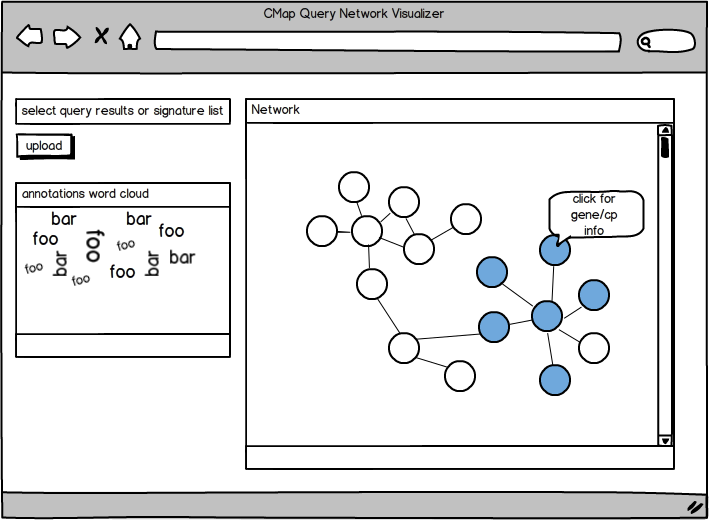
\includegraphics[scale=0.5]{img/app_mockup}
\caption{The App}
\label{fig:app_mockup}
\end{figure}

% methods
\section{Methods}
\subsection{Computing Connections}

Connections between CMap signatures will be computed using WTCS. In order to facilitate application performance, these connections will all be pre-computed and stored in a database. This way, the application can simply look up connectivity scores instead of computing them on-the-fly.

Users will interact with the application by inputting a list of signatures L that have resulted from running a CMap query. The application will sort L by the strength of connection to the user's query and then look up the connectivity scores between all pairwise combinations between the first N signatures within L, where N is a user-provided parameter. The application will then identify highly interconnected subsets of signatures by clustering the N signatures in pairwise connectivity space using k-means \cite{lloyd_least_squares_1982}. Additionally, it will compute the optimal number of clusters using the GAP statistic and will report the within cluster sum of squares (WCSS) for each cluster.

The N signatures will be displayed as a graph, where each signature is a node. Node pairs with non-zero connectivity scores will have edges drawn between them and nodes will be colored according to their cluster membership. This will allow users to easily visualize cluster concordance and relationships between clusters. The application will allow users to mouse-over nodes and see additional information about the signatures, such as the experimental parameters under which they were generated. The user will also be able to select a cluster or other user-defined group of nodes and see a word cloud generated from their annotations. The word cloud might give insight to pathway or pharmacological class membership for the nodes in question.

Finally, the application will support export of the clusters or user-defined groups of nodes into a text file for download.

\subsection{Software Components}
\subsubsection{Front End: HTML \& D3.js}

NEED REFERENCES FOR HTML STANDARD, JAVASCRIPT & D3

Hypertext markup language (HTML) is and has been the standard language for displaying information within web browsers. HTML5, the most recent revision of the HTML standard will be used as the framework of this application. To support user interaction, the graph and word cloud visualizations will be built using D3.js, a JavaScript library for data visualization.  

\subsubsection{Back End: Node.js \& MongoDB}

% challenges
\section{Potential Challenges}



% timeline
\section{Preliminary Timeline}
\begin{description}
\item[\date{2013-12-01}] Receive approval of proposal
\item[\date{2013-12-15}] Investigate and validate then notion of refining hit lists base on their interconnectivity
\item[\date{2013-12-22}] Implement graph visualizer in D3
\item[\date{2013-12-29}] Implement node selection and highlighting
\item[\date{2014-01-14}] Implement Node.js and MongoDB backend
\item[\date{2014-02-07}] Implement user-based input, uploading text files and CMap query results
\item[\date{2014-03-01}] Implement word-cloud generation based on selected graph nodes
\item[\date{2014-03-28}] Implement filtering, showing/hiding graph nodes, brushing to select nodes based on connectivity score
\item[\date{2014-04-15}] Implement text or spreadsheet result export
\item[\date{2014-05-01}] Implement linking to external sites (GeneBank, ChemBank, for clicking on graph nodes)
\end{description}

% bibliography
\bibliographystyle{apacite}
\bibliography{Proposal}

\end{document}